\documentclass[10pt, xetex, hyperref={pdfpagelabels=false}]{beamer}

% --------------------------------------------------------------------------
% Packages
% --------------------------------------------------------------------------
\usepackage[english]{babel}
\usepackage{amsmath, amsthm, amssymb}
\usepackage{bussproofs}
\EnableBpAbbreviations
\def\extraVskip{3pt}

\usepackage{fancyvrb}
\usepackage{geometry}
\usepackage{graphicx}
\usepackage{lmodern}

\usepackage{mylst}
\usepackage{url}

% --------------------------------------------------------------------------
% Tikz Configuration
% --------------------------------------------------------------------------
\usepackage{tikz}
\usetikzlibrary{positioning}
\usetikzlibrary{arrows}
\usetikzlibrary{automata}
\usetikzlibrary{calc}
\usepackage{rotating}

\tikzset{
    hyperlink node/.style={
        alias=sourcenode,
        append after command={
            let     \p1 = (sourcenode.north west),
                \p2=(sourcenode.south east),
                \n1={\x2-\x1},
                \n2={\y1-\y2} in
            node [inner sep=0pt, outer sep=0pt,anchor=north west,at=(\p1)]
            {\hyperlink{#1}{\XeTeXLinkBox{\phantom{\rule{\n1}{\n2}}}}}
                    %xelatex needs \XeTeXLinkBox, won't create a link unless it
                    %finds text --- rules don't work without \XeTeXLinkBox.
                    %Still builds correctly with pdflatex and lualatex
        }
    }
}

\tikzstyle{vertex}=[auto=left,circle,fill=black!25,minimum size=5pt,inner sep=0pt]

\newcommand{\gobackreconstruction}{
  \begin{tikzpicture}[overlay, remember picture, scale=0.5]
    \tikzset{shift={(current page.center)}, xshift=11.8cm,yshift=-8.4cm}
    \node[fill=plum,text=white, hyperlink node = reconstruction]
      (go) at (0,0) {\tiny Go Back};
  \end{tikzpicture}}


% --------------------------------------------------------------------------
% Color definitions.
% --------------------------------------------------------------------------
\usepackage{xcolor}
\definecolor{aliceblue}{rgb}{0.94, 0.97, 1.0}
\definecolor{amber}{rgb}{1.0, 0.75, 0.0}
\definecolor{amethyst}{rgb}{0.6, 0.4, 0.8}
\definecolor{antiquefuchsia}{rgb}{0.57, 0.36, 0.51}
\definecolor{ashgrey}{rgb}{0.7, 0.75, 0.71}
\definecolor{ballblue}{rgb}{0.13, 0.67, 0.8}
\definecolor{blue(munsell)}{rgb}{0.0, 0.5, 0.69}
\definecolor{blue(pigment)}{rgb}{0.2, 0.2, 0.6}
\definecolor{blu}{RGB}{1,0,102}
\definecolor{bondiblue}{rgb}{0.0, 0.58, 0.71}
\definecolor{brightmaroon}{rgb}{0.76, 0.13, 0.28}
\definecolor{cadet}{rgb}{0.33, 0.41, 0.47}

% --------------------------------------------------------------------------
% My palette.
% --------------------------------------------------------------------------
\definecolor{energy}{RGB}{49,247,250}
\definecolor{delicate}{RGB}{67,179,223}
\definecolor{faded}{RGB}{76,117,195}
\definecolor{plum}{RGB}{87,78,164}
\definecolor{petunias}{RGB}{109,80,139}
\definecolor{letour}{RGB}{101,41,105}
% --------------------------------------------------------------------------

% --------------------------------------------------------------------------
% Beamer configuration.
% --------------------------------------------------------------------------
\usetheme{default}
\usecolortheme{default}
\usefonttheme{serif}

\beamertemplatenavigationsymbolsempty
\setbeamertemplate{navigation symbols}{}
\hypersetup{pdfpagemode=UseNone}

% footer.
\setbeamercolor{headFoot}{fg=white, bg=plum!80!black}
\setbeamertemplate{footline}{
  \leavevmode%
  \hbox{%
  \begin{beamercolorbox}
    [wd=.8\paperwidth,ht=2.3ex,dp=1ex,left]{headFoot}%
    \hspace*{2ex}\textbf\insertshorttitle\hspace*{2mm}|
    \hspace*{2mm}\textbf\insertshortauthor
  \end{beamercolorbox}%
  \begin{beamercolorbox}
    [wd=.2\paperwidth,ht=2.3ex,dp=1ex,right]{headFoot}%
    \insertframenumber{}/\inserttotalframenumber\hspace*{2ex}
  \end{beamercolorbox}}%
  \vskip 0pt%
}

\setbeamerfont{frametitle}{size=\small,series=\bfseries}
\setbeamercolor{frametitle}{fg=white,bg=plum}

\setbeamerfont{framesubtitle}{size=\normalfont\scriptsize}
\setbeamercolor{framesubtitle}{fg=white, bg=plum!80!black}

\setbeamercolor{background canvas}{bg=white}
\setbeamercolor{normal text}{fg=black}

% \setbeamercolor{institute}{fg=blu}
\setbeamercolor{title}{fg=blu}
% \setbeamercolor{subtitle}{fg=blu}

% \setbeamercolor{titlelike}{fg=blu}
\setbeamerfont{footnote}{size=\tiny}
\setbeamercolor{footnote}{fg=gray}
% \setbeamercolor{block title}{bg=blue,fg=blu}
% \setbeamercolor{block body}{bg=aliceblue}
% \setbeamercolor{item}{fg=blu} % color of bullets
% \setbeamercolor{subitem}{fg=blu}
% \setbeamercolor{itemize/enumerate subbody}{fg=blu}
% \setbeamertemplate{itemize subitem}{{\textendash}}
% \setbeamerfont{itemize/enumerate subbody}{size=\footnotesize}
% \setbeamerfont{itemize/enumerate subitem}{size=\footnotesize}

% --------------------------------------------------------------------------
% Fonts
% --------------------------------------------------------------------------
\usefonttheme{professionalfonts}
\usefonttheme{serif}
\usepackage{fontspec}
\usepackage{mathtools}
\usepackage{unicode-math}

\newfontfamily\djvu[ExternalLocation=fonts/
  , BoldFont=DejaVuSansMono-Bold.ttf
  , BoldItalicFont=DejaVuSansMono-BoldOblique.ttf
  , ItalicFont=DejaVuSansMono-Oblique.ttf
  ]{DejaVuSansMono.ttf}

\setmonofont[ExternalLocation=fonts/
, BoldFont=DejaVuSansMono-Bold.ttf
, BoldItalicFont=DejaVuSansMono-BoldOblique.ttf
, ItalicFont=DejaVuSansMono-Oblique.ttf
]{DejaVuSansMono.ttf}

\setmathfont[ExternalLocation=fonts/
  ]{DejaVuMathTeXGyre.ttf}
\newfontfamily\mathfont{fonts/DejaVuMathTeXGyre.ttf}

\setmainfont[ExternalLocation=fonts/
  , BoldFont=SourceSansPro-Semibold.otf
  , BoldItalicFont=SourceSansPro-SemiboldIt.otf
  , ItalicFont=SourceSansPro-It.otf
  ]{SourceSansPro-Regular.otf}

% \setmonofont[ExternalLocation=fonts/
%   , BoldFont=SourceCodePro-Semibold.ttf
%   , BoldItalicFont=SourceCodePro-SemiboldIt.ttf
%   , ItalicFont=SourceCodePro-It.ttf
%   ]{SourceCodePro-Regular.ttf}

\newfontfamily\sourcecode[ExternalLocation=fonts/
  , BoldFont=SourceCodePro-Semibold.ttf
  , BoldItalicFont=SourceCodePro-SemiboldIt.ttf
  , ItalicFont=SourceCodePro-It.ttf
  ]{SourceCodePro-Regular.ttf}


\usepackage{minted}
\setminted[cagda]{
  bgcolor   = aliceblue
, fontsize  = \footnotesize
, frame     = none
% , framerule = 0.4pt
% , framesep  = 0pt
, style     = cagda
}


% --------------------------------------------------------------------------
% References
% --------------------------------------------------------------------------

\usepackage[autostyle]{csquotes}
\usepackage[
    backend=biber
  , doi=false
  , eprint=false
  , isbn=false
  , natbib=true
  , sortlocale=en_US
  , style=authoryear-icomp
  , url=true
]{biblatex}
\addbibresource{ref.bib}
\renewcommand*{\nameyeardelim}{\addcomma\addspace}
\usepackage{silence}
\WarningFilter{biblatex}{Patching footnotes failed}
\WarningFilter{hyperref}{Token not allowed in a PDF string}

% --------------------------------------------------------------------------
% Title and Author
% --------------------------------------------------------------------------

\title[Proof Reconstruction in Classical Propositional Logic]
  {\textbf{Proof Reconstruction in Classical Propositional Logic}}
\subtitle{(work in progress)}
\date{May 11, 2017\\Updated: \today}
\author[Jonathan Prieto-Cubides]{Jonathan Prieto-Cubides\\
(joint work with Andr\'es Sicard-Ram\'irez)}
\institute{
Master in Applied Mathematics\\
Universidad EAFIT\\
Medell\'in, Colombia}
% --------------------------------------------------------------------------

\newsavebox\agdapragma

\begin{document}
\setcounter{page}{1}

\begin{frame}[plain]
\titlepage
  \begin{tikzpicture}[overlay, remember picture]
   \tikzset{shift={(current page.center)}}
    \node[xshift=-4.7cm,yshift=-3.2cm] (eafit)
      {
\includegraphics[width=0.2\textwidth]{figures/eafit}};
    \node[xshift=4.7cm,yshift=-3cm] (chalmers)
      {
\includegraphics[width=0.17\textwidth]{figures/chalmers}};
  \end{tikzpicture}
\end{frame}

\begin{frame}[fragile]{Proof Reconstruction: Overview}
\vfill
\begin{tikzpicture}
\node(problem) at (0,0)
   {
\includegraphics[scale=0.7]{figures/problem}};
\node[right = 0.8cm of problem, hyperlink node=tptp-syntax](tptp){

\includegraphics[scale=0.7]{figures/tptp}
};
\node[right= 0.8cm of tptp, hyperlink node=metis] (metis)
  {
\includegraphics[scale=0.7]{figures/metis}};
\node[right= 0.8cm of metis, hyperlink node=tstp-syntax] (tstp)
  {
\includegraphics[scale=0.7]{figures/tstp}};
\node[below= 1.5cm of tstp, hyperlink node=athena] (athena)
  {
\includegraphics[scale=0.7]{figures/athena}};
\node[left = 0.6cm of athena, hyperlink node=agda-file] (agdafile)
  {
\includegraphics[scale=0.7]{figures/agdafile}};
\node[left = 0.5cm of agdafile] (agda)
  {
\includegraphics[scale=0.7]{figures/agda}};
\node[below = 0.18cm of problem, hyperlink node=verified-example] (verified)
  {
\includegraphics[scale=0.7]{figures/verified}};
\node[below = 0.18cm of verified, opacity=0.5, hyperlink node=failure-example] (failure)
  {
\includegraphics[scale=0.7]{figures/failure}};

\draw[->, thick] (problem) to (tptp);
\draw[->, thick] (tptp) to (metis);
\draw[->, thick] (metis) to (tstp);
\draw[->, thick] (tstp) to (athena);
\draw[->, thick] (athena) to (agdafile);
\draw[->, thick] (agdafile) to (agda);
\draw[->, thick] (agda) to (verified);
\draw[->, thick, gray] (agda) to (failure);
\end{tikzpicture}
\vfill
\end{frame}


% Now each step paused.

\begin{frame}[fragile, label=overview]{Proof Reconstruction: Overview}
\vfill
\begin{tikzpicture}
\only<1->{\node(problem) at (0,0)
 {
\includegraphics[scale=0.7]{figures/problem}};
}

\only<2->{\node[right = 0.8cm of problem, hyperlink node=tptp-syntax](tptp){

\includegraphics[scale=0.7]{figures/tptp}
};
}
\only<3->{
\node[right= 0.8cm of tptp, hyperlink node=metis] (metis)
  {
\includegraphics[scale=0.7]{figures/metis}\,
  \footnote{\url{http://www.gilith.com/software/metis}.}
  };
}
\only<4->{
\node[right= 0.8cm of metis, hyperlink node=tstp-syntax] (tstp)
  {
\includegraphics[scale=0.7]{figures/tstp}};
}
\only<5->{
\node[below= 1.5cm of tstp, hyperlink node=athena] (athena)
  {
\includegraphics[scale=0.7]{figures/athena}
  \footnote{\url{http://github.com/jonaprieto/athena}.}
  };
}
\only<6->{
\node[left = 0.6cm of athena, hyperlink node=agda-file] (agdafile)
  {
\includegraphics[scale=0.7]{figures/agdafile}
  };
}
\only<7->{
\node[left = 0.5cm of agdafile] (agda)
  {
\includegraphics[scale=0.7]{figures/agda}
  \footnote{\url{http://github.com/agda/agda}.}
  };
}
\only<8->{
\node[below = 0.18cm of problem, hyperlink node=verified-example] (verified)
  {
\includegraphics[scale=0.7]{figures/verified}};
}
\only<9->{
\node[below = 0.18cm of verified, opacity=0.5, hyperlink node=failure-example] (failure)
  {
\includegraphics[scale=0.7]{figures/failure}};
}

\only<2->{ \draw[->, thick] (problem) to (tptp)};
\only<3->{ \draw[->, thick] (tptp) to (metis)};
\only<4->{ \draw[->, thick] (metis) to (tstp)};
\only<5->{ \draw[->, thick] (tstp) to (athena)};
\only<6->{ \draw[->, thick] (athena) to (agdafile)};
\only<7->{ \draw[->, thick] (agdafile) to (agda)};
\only<8->{ \draw[->, thick] (agda) to (verified)};
\only<9->{ \draw[->, thick, gray] (agda) to (failure)};
\end{tikzpicture}
\vfill
\end{frame}

\begin{frame}{Obstacles to Reconstruction with Automatic Provers \citep{Paulson2007}}
\begin{itemize}
\item \textit{Ambiguities}: their output typically omits crucial information,
such as which term is affected by rewriting.
\item \textit{Lack of standards}: automatic provers generate different output formats
and employ a variety of inference systems
\item \textit{Complexity}: a single automatic prover may use numerous inference rules with
complicated behaviors
\item \textit{Problem transformations}: ATPs re-order literals and make other changes to the clauses
they are given
\end{itemize}

\end{frame}

\begin{frame}[fragile, label=reconstruction]{Proof Reconstruction: Overview}
\vfill
\begin{tikzpicture}
\node(problem) at (0,0)
   {
\includegraphics[scale=0.7]{figures/problem}};
\node[right = 0.8cm of problem, hyperlink node=tptp-syntax](tptp){

\includegraphics[scale=0.7]{figures/tptp}
};
\node[right= 0.8cm of tptp, hyperlink node=metis] (metis)
  {
\includegraphics[scale=0.7]{figures/metis}};
\node[right= 0.8cm of metis, hyperlink node=tstp-syntax] (tstp)
  {
\includegraphics[scale=0.7]{figures/tstp}};
\node[below= 1.5cm of tstp, hyperlink node=athena] (athena)
  {
\includegraphics[scale=0.7]{figures/athena}};
\node[left = 0.6cm of athena, hyperlink node=agda-file] (agdafile)
  {
\includegraphics[scale=0.7]{figures/agdafile}};
\node[left = 0.5cm of agdafile] (agda)
  {
\includegraphics[scale=0.7]{figures/agda}};
\node[below = 0.18cm of problem, hyperlink node=verified-example] (verified)
  {
\includegraphics[scale=0.7]{figures/verified}};
\node[below = 0.18cm of verified, opacity=0.5, hyperlink node=failure-example] (failure)
  {
\includegraphics[scale=0.7]{figures/failure}};

\draw[->, thick] (problem) to (tptp);
\draw[->, thick] (tptp) to (metis);
\draw[->, thick] (metis) to (tstp);
\draw[->, thick] (tstp) to (athena);
\draw[->, thick] (athena) to (agdafile);
\draw[->, thick] (agdafile) to (agda);
\draw[->, thick] (agda) to (verified);
\draw[->, thick, gray] (agda) to (failure);
\end{tikzpicture}
\vfill
\end{frame}

\begin{frame}[fragile, label=tptp-syntax]{\texttt{TPTP} Syntax}
  {Thousands of Problems for Theorem Provers}

 \tikz[overlay,remember picture]
  \node at (0.92\textwidth, 0cm)
    {
\includegraphics[width=0.15\textwidth]{figures/tptp}};

  \begin{itemize}
  \item Is a language\footnote{\url{http://www.cs.miami.edu/~tptp/TPTP/SyntaxBNF.html}.}
        to encode problems \citep{Sut09}
  \item Is the input of the ATPs
  \item Annotated formulas with the form
   \begin{center}
\begin{tptp}
language(name, role, formula).
\end{tptp}
    \end{center}
    \begin{itemize}
      \item[\texttt{language}] FOF or CNF
      \item[\texttt{name}] to identify the formula within the problem
      \item[\texttt{role}] axiom, definition, hypothesis, conjecture
      \item[\texttt{formula}] formula in \texttt{TPTP} format
    \end{itemize}
  \end{itemize}
\end{frame}

\begin{frame}[fragile, label=tptp-examples]{\texttt{TPTP} Examples}

\begin{itemize}
  \item $p ⊢ p$
\begin{tptp}
fof(myaxiom, axiom, p).
fof(goal, conjecture, p).
\end{tptp}

  \item $⊢ ¬ (p ∧ ¬ p) ∨ (q ∧ ¬ q)$
\begin{tptp}
fof(goal, conjecture, ~ ((p & ~ p) | (q & ~ q))).
\end{tptp}
  \end{itemize}
\gobackreconstruction
\end{frame}

\begin{frame}[label=metis]{\texttt{Metis} Theorem Prover
  \footnote{\url{http://www.gilith.com/software/metis/}.}}
 \tikz[overlay,remember picture]
  \node at (0.92\textwidth, 0.5cm)
    {
\includegraphics[width=0.15\textwidth]{figures/metis}};

\texttt{Metis} is an automatic theorem prover for First-Order Logic with Equality
\citep{hurd2003first}
\begin{block}{Why Metis?}
  \begin{itemize}
    \item \href{https://github.com/gilith/metis}{Open source} implemented in
       \texttt{Standard ML}
    \item Each refutation step is one of
      \hyperlink{metis-inference-rules}{\textit{six rules}}
    \item Reads problem in \hyperlink{tptp-syntax}{\texttt{TPTP} format}
    \item Outputs \textit{detailed} proofs in \hyperlink{tstp-syntax}{\texttt{TSTP} format}
  \end{itemize}
\end{block}
\end{frame}


\begin{frame}[fragile, label=metis-rules]{Inference Rules of \texttt{Metis}}
\hyperlink{tstp-example}{\texttt{TSTP}} derivations by \texttt{Metis} exhibit these inferences\footnote{Inference rules found in proofs of Propositional Logic theorems.}
\vfill
\begin{table}[!ht]
\begin{center}
\scalebox{0.8}{
{\renewcommand{\arraystretch}{1.3}%
\begin{tabular}{|ll| }
\hline
\textbf{Rule} & \textbf{Purpose} \\
\hline
\texttt{canonicalize} & transforms formulas to CNF, DNF or NNF\\
\texttt{clausify} & performs clausification\\
\hyperlink{atp-conjunct}{\texttt{conjunct}} & takes a formula from a conjunction\\
\texttt{negate} & applies negation to the formula\\
\texttt{resolve} & applies theorems of resolution\\
\texttt{simplify} & applies over a list of formula to simplify them\\
\texttt{strip} & splits a formula into subgoals\\[1ex]
\hline
\end{tabular}}
}
\end{center}
\label{tab:label}
\end{table}
\vfill
\gobackreconstruction
\end{frame}

\begin{frame}[fragile, label=tstp-syntax]{\texttt{TSTP} Syntax}

 \tikz[overlay,remember picture]
  \node at (0.92\textwidth, -0.5cm)
    {
\includegraphics[width=0.15\textwidth]{figures/tstp}};

A \texttt{TSTP} derivation\footnote{\url{http://www.cs.miami.edu/~tptp/TPTP/QuickGuide/Derivations.html}.}
\begin{itemize}
  \item Is a \hyperlink{tstp-dag}{\textbf{D}irected \textbf{A}cyclic \textbf{G}raph} where
  \begin{itemize}
    \item[\texttt{leaf}] is a formula from the \hyperlink{tptp-syntax}{\texttt{TPTP}} input
    \item[\texttt{node}] is a formula inferred from parent formula
    \item[\texttt{root}] the final derived formula
  \end{itemize}
  \item Is a list of annotated formulas with the form
  \end{itemize}

\begin{center}
  {\footnotesize
\begin{tptp}
language(name, role, formula, source [,useful info]).
\end{tptp}}
\end{center}

where \texttt{\color{plum} source} typically is an inference record
\begin{center}
{\footnotesize
\begin{tptp}
inference(rule, useful info, parents).
\end{tptp}
}
\end{center}
\end{frame}

\begin{frame}[fragile, label=tstp-example]{\texttt{TSTP} Example}

 % \tikz[overlay,remember picture]
 %  \node at (0.93\textwidth, -0.3cm)
 %    {
\includegraphics[width=0.15\textwidth]{figures/metis}};

\begin{itemize}
  \item Proof found by \texttt{Metis} for the problem $p ⊢ p$
{\small
\begin{tptp}
$ metis --show proof problem.tptp
fof(a, axiom, p).
fof(goal, conjecture, p).
fof(subgoal_0, plain, p),
  inference(strip, [], [goal])).
fof(negate_0_0, plain, ~ p,
  inference(negate, [], [subgoal_0])).
fof(normalize_0_0, plain, ~ p,
  inference(canonicalize, [], [negate_0_0])).
fof(normalize_0_1, plain, p,
  inference(canonicalize, [], [a])).
fof(normalize_0_2, plain, $false,
  inference(simplify, [],
    [normalize_0_0, normalize_0_1])).
cnf(refute_0_0, plain, $false,
    inference(canonicalize, [], [normalize_0_2])).
\end{tptp}
}
\end{itemize}
\end{frame}


\begin{frame}[fragile, label=tstp-dag]{DAG Example}
\vfill
By refutation, we proved $p ⊢ p$:

\begin{columns}
\begin{column}{0.5\textwidth}

\begin{prooftree}
\AxiomC{}
\RightLabel{\texttt{\scriptsize assume}}
\UnaryInfC{$¬ p$}
\RightLabel{\texttt{\scriptsize strip}}
\UnaryInfC{$¬ p$}
\AxiomC{}
\RightLabel{\texttt{\scriptsize axiom}}
\UnaryInfC{$p$}
\RightLabel{\texttt{\scriptsize canonicalize}}
\UnaryInfC{$p$}
\RightLabel{\texttt{\scriptsize simplify}}
\BinaryInfC{$⊥$}
\RightLabel{\texttt{\scriptsize canonicalize}}
\UnaryInfC{$⊥$}
\end{prooftree}
\end{column}
\begin{column}{0.5\textwidth}  %%<--- here
    \begin{center}
    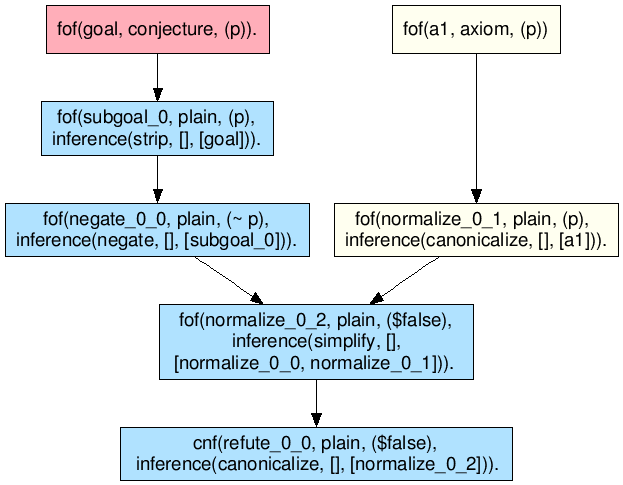
\includegraphics[height=0.8\textwidth]{figures/derivation.png}
     \end{center}
\end{column}
\end{columns}
\vfill
\gobackreconstruction
\end{frame}


\begin{frame}[fragile, label=athena]{\texttt{Athena}~\citep{Athena}}

 \begin{tikzpicture}[overlay,remember picture]
 \tikzset{shift={(current page.north)}, xshift=0cm,yshift=0cm}
  \node[] at (0.92\textwidth, 1cm)
    {
\includegraphics[width=0.15\textwidth]{figures/athena}};
\end{tikzpicture}

Is a \texttt{Haskell} program
that translates proofs given by \texttt{Metis}
in \texttt{TSTP} format to \texttt{Agda} code\\

\begin{itemize}
    \item Parsing of \texttt{TSTP} language\footnote{\label{parsing}\url{https://github.com/agomezl/tstp2agda}.}
    \item Creation\textsuperscript{\ref{parsing}} and analysis of \hyperlink{tstp-dag}{\textbf{DAG}} derivations
    \item Analysis of inference rules used in the \texttt{TSTP} derivation
    \item \texttt{Agda} code generation
\begin{table}[!ht]
\begin{center}
\scalebox{0.8}{
{\renewcommand{\arraystretch}{1.3}%
\begin{tabular}{|ll| }
\hline
\textbf{Library} & \textbf{Purpose} \\
\hline
\texttt{\hyperlink{agda-prop}{\texttt{Agda-Prop}}}& axioms and theorems of Classical Propositional Logic\\
\texttt{\hyperlink{agda-metis}{\texttt{Agda-Metis}}} & versions of the inference rules used by \texttt{Metis}\\
\hline
\end{tabular}}
}
\end{center}
\label{tab:library}
\end{table}

\end{itemize}
\end{frame}

\begin{frame}[fragile, label=agda-prop-2]{\texttt{Agda-Prop} Library
  \footnote{\url{https://github.com/jonaprieto/agda-prop}.}}
\begin{itemize}
  \item Intuitionistic Propositional Logic + PEM ($Γ ⊢ ϕ ∨ ¬ ϕ$)
  \item A data type for formulas
  \vspace*{1mm}

\begin{minted}{cagda}
data Prop : Set where
  Var : Fin n → Prop
  ⊤   : Prop
  ⊥   : Prop
  _∧_ : (φ ψ : Prop) → Prop
  _∨_ : (φ ψ : Prop) → Prop
  _⇒_ : (φ ψ : Prop) → Prop
  _⇔_ : (φ ψ : Prop) → Prop
  ¬_  : (φ : Prop)   → Prop
\end{minted}
\end{itemize}
\end{frame}

\begin{frame}[fragile, label=agda-prop]{\texttt{Agda-Prop} Library~\citep{AgdaProp}}
\begin{itemize}
  \item A data type for theorems
  \vspace*{1mm}
\begin{minted}{cagda}
data _⊢_ : (Γ : Ctxt)(φ : Prop) → Set
\end{minted}

\item Constructors
  \vspace*{1mm}

\begin{minted}{cagda}
assume, axiom, weaken, ⊤-intro, ⊥-elim, ¬-intro,
¬-elim, ∧-intro, ∧-proj₁, ∧-proj₂, ∨-intro₁,
∨-intro₂, ∨-elim, ⇒-intro, ⇒-elim, ⇔-intro,
⇔-elim₁, ⇔-elim₂.
\end{minted}
  \item Natural deduction proofs for more than 71 theorems
  \vspace*{1mm}
\begin{minted}{cagda}
⇔-equiv, ⇔-assoc, ⇔-comm, ⇒-⇔-¬∨, ⇔-¬-to-¬,
¬⇔-to-¬, ¬¬-equiv, ⇒⇒-⇔-∧⇒, ⇔-trans, ∧-assoc,
∧-comm, ∧-dist, ¬∧-to-¬∨¬, ¬∨¬-to-¬∧, ¬∨¬-⇔-¬∧,
subst⊢∧₁, subst⊢∧₂, ∨-assoc, ∨-comm, ∨-dist,
∨-equiv, ¬∨-to-¬∧¬, ¬∧¬-to-¬∨, ∨-dmorgan,
¬¬∨¬¬-to-∨, cnf, nnf, dnf, RAA, ...
\end{minted}
\end{itemize}
\end{frame}


\begin{frame}[fragile, label=agda-metis]{\texttt{Agda-Metis} Library
  ~\citep{AgdaMetis}}
\vfill
\begin{table}[!ht]
\begin{center}
\scalebox{0.7}{
{\renewcommand{\arraystretch}{1.3}%
\begin{tabular}{|lll|}
\hline
\textbf{Rule} & \textbf{Purpose} &\textbf{Theorem}\\
\hline
\texttt{canonicalize} & transforms formulas to CNF, DNF or NNF &\texttt{atp-canonicalize}\\
\texttt{clausify} & performs clausification &\texttt{atp-clausify}\\
\hyperlink{atp-conjunct}{\texttt{conjunct}} & takes a formula from a conjunction &\hyperlink{atp-conjunct}{\texttt{atp-conjunct}}\\
\texttt{negate} & append negation symbol to the formula &\texttt{atp-negate}\\
\texttt{resolve} & applies theorems of resolution &\texttt{atp-resolve}\\
\texttt{simplify} & applies over a list of formula to simplify them &\texttt{atp-simplify}\\
\texttt{strip} & splits a formula into subgoals &\texttt{atp-strip}\\[1ex]
\hline
\end{tabular}}
}
\end{center}
\label{tab:agda-metis-table}
\end{table}
\vfill
\end{frame}


\begin{frame}[fragile, label=atp-conjunct]{\texttt{Agda-Metis}: Conjunct Inference
  \footnote{\url{https://github.com/jonaprieto/agda-metis}.}
  }

\vfill
\begin{itemize}
\item Definition
\begin{equation*}
\text{\color{plum!40!black}conjunct}(\overbrace{\varphi_1 ∧ ⋯ ∧ \varphi_n}^{\varphi}, \psi)
= \begin{cases}
\varphi_{i} \ \ \ \ \text{if }\psi\text{ is equal to some }\varphi_i\\
\varphi    \ \ \ \ \text{otherwise}
\end{cases}
\end{equation*}

\pause
\item Inference rules involved
\begin{center}
\begin{columns}
\begin{column}{0.42\textwidth}

 \begin{prooftree}
  \AxiomC{$\varphi_1 ∧ \varphi_2$}
  \RightLabel{\scriptsize $∧$-\texttt{proj}$₁$}
  \UnaryInfC{$\varphi_1$}
  \end{prooftree}
\end{column}

\begin{column}{0.42\textwidth}
 \begin{prooftree}
  \AxiomC{$\varphi_1 ∧ \varphi_2$}
  \RightLabel{\scriptsize $∧$-\texttt{proj}$₂$}
  \UnaryInfC{$\varphi₂$}
  \end{prooftree}
\end{column}

\begin{column}{0.2\textwidth}  %%<--- here
  \begin{tikzpicture}[
    ->
  , >=stealth'
  , shorten >=1pt
  , auto
%  , node distance=2.8cm
  , thick
  , every state/.style={fill=plum!45!black,draw=none,text=white}
  , overlay
  , remember picture
    , transform canvas={scale=.75}
    ]
  \tikzset{shift={(current page.center)}, xshift=4.5cm,yshift=0cm}
    

  \node[state]  (phi)                     {$\varphi$};
  \node[state]  (phi1) [below left =1.3cm and 0.1cm of phi]  {$\varphi_1$};
  \node[state]  (phi2) [below right=1.3cm and 0.1cm of phi]  {$\varphi_2$};
  \node[state]  (phi3)  [below left =1.3cm and 0.1cm of phi2]  {$\varphi_3$};
  \node[state]  (phi4)  [below right =1.3cm and 0.1cm of phi2]  {$\varphi_4$};

  \path[every node/.style={sloped,anchor=south,auto=false}]
        (phi) edge node {\tiny $∧$-\texttt{proj}$₁$} (phi1)            
        (phi) edge node {\tiny $∧$-\texttt{proj}$₂$} (phi2)
        (phi2) edge node {\tiny $∧$-\texttt{proj}$₁$} (phi3)
        (phi2) edge node {\tiny $∧$-\texttt{proj}$₂$} (phi4);

\end{tikzpicture}
\end{column}
\end{columns}
\end{center}
\vskip 2mm

\item Example
\[ \varphi := \varphi_1 ∧ \overbrace{(\varphi_3 ∧ \varphi_4)}^{\varphi_2}\]

\begin{itemize}

\item
\texttt{conjunct}$(\varphi , \varphi_3 ∧ \varphi_1) ≡ \varphi$
\vskip 3mm
\item
\texttt{conjunct}$(\varphi , \varphi_3)      ≡ \varphi_3$
\vskip 3mm
\item
\texttt{conjunct}$(\varphi , \varphi_2)      ≡ \varphi_2$
\vskip 3mm
\end{itemize}

\end{itemize}
\end{frame}

\begin{frame}[fragile]

\begin{minted}{cagda}
data ConjView : Prop → Set where
  conj  : (φ₁ φ₂ : Prop) → ConjView (φ₁ ∧ φ₂)
  other : (φ : Prop)     → ConjView φ

conj-view : (φ : Prop) → ConjView φ
conj-view (φ ∧ ψ) = conj _ _
conj-view φ       = other _

data Step : Set where
  pick  : Step
  proj₁ : Step
  proj₂ : Step

Path : Set
Path = List Step

conjunct-path : (φ ψ : Prop) → Path → Path
conjunct-path φ ψ path with ⌊ eq φ ψ ⌋
... | true  = path ∷ʳ pick
... | false with conj-view φ
...   | other _ = []
...   | conj φ₁ φ₂ with conjunct-path φ₁ ψ []
...     | subpath@(_ ∷ _) = (path ∷ʳ proj₁) ++ subpath
...     | [] with conjunct-path φ₂ ψ []
...          | subpath@(_ ∷ _) = (path ∷ʳ proj₂) ++ subpath
...          | []              = []
\end{minted}

\end{frame}


\begin{frame}[fragile, label=atp-conjunct-proof]{The \texttt{conjunct} function and its theorem, \texttt{atp-conjunct}}
\vfill
\begin{minted}{cagda}
conjunct : (φ ψ : Prop) → Prop
conjunct φ ψ with conj-view φ | conjunct-path φ ψ []
... | _          | []        = φ
... | conj _ _   | pick  ∷ _ = φ
... | conj φ₁ _  | proj₁ ∷ _ = conjunct φ₁ ψ
... | conj _ φ₂  | proj₂ ∷ _ = conjunct φ₂ ψ
... | other .φ   | _         = φ

atp-conjunct
  : ∀ {Γ} {φ}
  → (ψ : Prop)
  → Γ ⊢ φ
  → Γ ⊢ conjunct φ ψ

atp-conjunct {Γ} {φ} ψ Γ⊢φ
  with conj-view φ | conjunct-path φ ψ []
...  | _           | []        = Γ⊢φ
...  | conj _ _    | pick  ∷ _ = Γ⊢φ
...  | conj _ _    | proj₁ ∷ _ = atp-conjunct ψ (∧-proj₁ Γ⊢φ)
...  | conj _ _    | proj₂ ∷ _ = atp-conjunct ψ (∧-proj₂ Γ⊢φ)
...  | other _     | (_ ∷ _)   = Γ⊢φ
\end{minted}
\vfill
\gobackreconstruction
\end{frame}

\begin{frame}[fragile, label=agda-file]{\texttt{Agda} Code Example}
  {Generated by \texttt{Athena} Tool}

\begin{itemize}
  \item The problem is $p ∧ q ⊢ q ∧ p$
  \item In \texttt{TPTP} format
\begin{tptp}
$ cat problem.tptp
fof(a, axiom, p & q).
fof(goal, conjecture, q & p).
\end{tptp}
  \item How to use Athena with your problem

\begin{tptp}
$ metis --show proof problem.tptp > problem.tstp
$ athena problem.tstp
$ agda problem.tstp
\end{tptp}
\end{itemize}
\end{frame}

\begin{frame}[fragile, allowframebreaks]{\texttt{TSTP} Derivation given by \texttt{Metis}}
\begin{tptp}
fof(a, axiom, p & q).
fof(goal, conjecture, q & p).
fof(subgoal_0, plain, q,
    inference(strip, [], [goal])).
fof(subgoal_1, plain, q => p,
    inference(strip, [], [goal])).
fof(negate_0_0, plain, ~ q,
inference(negate, [], [subgoal_0])).
fof(normalize_0_0, plain, (~ q),
    inference(canonicalize, [], [negate_0_0])).
fof(normalize_0_1, plain, p & q,
    inference(canonicalize, [], [a])).
fof(normalize_0_2, plain, q,
    inference(conjunct, [], [normalize_0_1])).
fof(normalize_0_3, plain, $false,
    inference(simplify, [],
        [normalize_0_0, normalize_0_2])).
cnf(refute_0_0, plain, $false,
    inference(canonicalize, [], [normalize_0_3])).
fof(negate_1_0, plain, ~ (q => p),
    inference(negate, [], [subgoal_1])).
fof(normalize_1_0, plain, ~ p & q,
    inference(canonicalize, [], [negate_1_0])).
fof(normalize_1_1, plain, p & q,
     inference(canonicalize, [], [a])).
fof(normalize_1_2, plain, p,
    inference(conjunct, [], [normalize_1_1])).
fof(normalize_1_3, plain, q,
    inference(conjunct, [], [normalize_1_1])).
fof(normalize_1_4, plain, $false,
    inference(simplify, [],
      [normalize_1_0, normalize_1_2, normalize_1_3])).
cnf(refute_1_0, plain, ($false),
    inference(canonicalize, [], [normalize_1_4])).
\end{tptp}
\end{frame}

\begin{frame}[fragile, label=verified-example]{Problem $p ∧ q ⊢ q ∧ p$}{Reconstructed Proof generated with \texttt{Athena}}
\vfill
\begin{minted}{cagda}
p, q, a, goal, subgoal₀, subgoal₁ : Prop

-- Axiom.
a = p ∧ q

-- Premise.
Γ : Ctxt
Γ = [ a ]

-- Conjecture.
goal = q ∧ p

-- Subgoals.
subgoal₀ = q
subgoal₁ = q ⇒ p
\end{minted}
\vfill
\end{frame}

\begin{frame}[fragile, label=verified-example-2]{Problem $p ∧ q ⊢ q ∧ p$}{Reconstructed Proof}
\vfill
\begin{minted}{cagda}
a : Prop
a = p ∧ q

subgoal₀ : Prop
subgoal₀ = q

proof₀ : Γ ⊢ subgoal₀
proof₀ =
  (RAA
    (atp-canonicalize
      (atp-simplify
        (atp-canonicalize
          (atp-strip
            (assume {Γ = Γ} (atp-negate subgoal₀))))
        (atp-conjunct (q)
          (atp-canonicalize
            (weaken (atp-negate subgoal₀)
              (assume {Γ = ∅} a)))))))
\end{minted}
\vfill
\end{frame}

\begin{frame}[fragile, label=verified-example-3]{Problem $p ∧ q ⊢ q ∧ p$}{Reconstructed Proof}
\vfill
\begin{minted}{cagda}
subgoal₁ : Prop
subgoal₁ = q ⇒ p

proof₁ : Γ ⊢ subgoal₁
proof₁ =
  (RAA
    (atp-canonicalize
      (atp-simplify
        (atp-conjunct (q)
          (atp-canonicalize
            (weaken (atp-negate subgoal₁)
              (assume {Γ = ∅} a))))
        (atp-simplify
          (atp-canonicalize
            (atp-strip
              (assume {Γ = Γ} (atp-negate subgoal₁))))
          (atp-conjunct (p)
            (atp-canonicalize
              (weaken (atp-negate subgoal₁)
                (assume {Γ = ∅} a))))))))
\end{minted}
\vfill
\end{frame}

\begin{frame}[fragile, label=verified-example-4]{Problem $p ∧ q ⊢ q ∧ p$}{Reconstructed proof}
\vfill
\begin{minted}{cagda}
-- Premise.
Γ = [ a ]

-- Conjecture.
goal = q ∧ p

-- Subgoals.
subgoal₀ = q
subgoal₁ = q ⇒ p

-- Proof
proof₀ : Γ ⊢ subgoal₀
proof₁ : Γ ⊢ subgoal₁

proof : Γ ⊢ goal
proof =
  ⇒-elim
    atp-splitGoal            -- q ∧ (q ⇒ p) ⇒ p
    (∧-intro proof₀ proof₁)
\end{minted}
\vfill
\gobackreconstruction
\end{frame}

\begin{frame}[fragile, label=failure-example]{Bug\footnote{\url{https://github.com/gilith/metis/issues/2}.} in the Printing of the Proof}
  {\texttt{Metis} v2.3 (release 20161108)}
% {}
\begin{tptp}
$ cat problem.tptp
fof(goal, conjecture,
  ((p <=> q) <=> r) <=> (p <=> (q <=> r))).
\end{tptp}
\begin{tptp}
$ metis --show proof problem.tptp
...
fof(normalize_2_0, plain,
  (~ p & (~ q <=> ~ r) & (~ p <=> (~ q <=> ~ r))),
  inference(canonicalize, [], [negate_2_0])).
fof(normalize_2_1, plain, ~ p <=> (~ q <=> ~ r),
    inference(conjunct, [], [normalize_2_0])).
fof(normalize_2_2, plain, ~ q <=> ~ r,
    inference(conjunct, [], [normalize_2_0])).
fof(normalize_2_3, plain, ~ p,
  inference(conjunct, [], [normalize_2_0])).
fof(normalize_2_4, plain, $false,
    inference(simplify, [],
      [normalize_2_1, normalize_2_2, normalize_2_3])).
...
\end{tptp}
\end{frame}

\begin{frame}[fragile, label=failure-example-2]{Bug in the Printing of the Proof}
  {\texttt{Metis} v2.3 (release 20161108)}

\[ φ := ¬ p ∧ (¬ q ⇔ ¬ r) ∧ (¬ p ⇔ (¬ q ⇔ ¬ r))\]

\begin{prooftree}
\AxiomC{$\vdots$}
\RightLabel{\scriptsize{canonicalize}}
\UnaryInfC{$φ$}
\RightLabel{\scriptsize{conjunct}}
\UnaryInfC{$¬ p ⇔ (¬ q ⇔ ¬ r)$}

\AxiomC{$\vdots$}
\RightLabel{\scriptsize{canonicalize}}
\UnaryInfC{$φ$}
\RightLabel{\scriptsize{conjunct}}
\UnaryInfC{$¬ q ⇔ ¬ r$}

\AxiomC{$\vdots$}
\RightLabel{\scriptsize{canonicalize}}
\UnaryInfC{$φ$}
\RightLabel{\scriptsize{conjunct}}
\UnaryInfC{$¬ p$}

\RightLabel{\scriptsize{simplify}}
\TrinaryInfC{$\bot$}
\end{prooftree}
\pause
The bug was caused by the conversion of \texttt{Xor} sets to \texttt{Iff} lists.
After reporting this, Hurd fixed the printing of \texttt{canonicalize} inference rule
\[ φ := ¬ p ∧ (¬ q ⇔ ¬ r) ∧ (¬ p ⇔ (¬ q ⇔ {\color{red} r}))\]
\gobackreconstruction
\end{frame}


\begin{frame}[fragile, label=hammer]{Related Work}
\begin{block}{SledgeHammer} \citep{Paulson2007}
\begin{itemize}
\item \texttt{Isabelle}/\texttt{HOL} mature tool
\item \texttt{Metis} ported within \texttt{Isabelle/HOL}
\item Reconstruct proofs of well-known ATPs: \texttt{EProver}, \texttt{Vampire},
among others using \texttt{SystemOnTPTP} server
\end{itemize}
\end{block}

\begin{block}{Integrating \texttt{Waldmeister} into \texttt{Agda}} \citep{Foster2011}
\begin{itemize}
  \item Framework for a integration between \texttt{Agda} and ATPs
  \begin{itemize}
    \item Equational Logic
    \item Reflection Layers
  \end{itemize}
  \item Source code is not available\footnote{\url{http://simon-foster.staff.shef.ac.uk/agdaatp}.}
  \end{itemize}
\end{block}
\end{frame}



\begin{frame}[fragile]{Related Work: \texttt{Apia}}
  {Proving First-Order theorems written in \texttt{Agda} using automatic
  theorem provers for First-Order Logic}

\only<1>{At the moment, the communication between \texttt{Agda} and
the ATPs is unidirectional because the ATPs are being used as oracles \citep{Sicard2015}
\vfill
}
\only<1>{
\inputminted{cagda}{Or.agda}
\begin{tikzpicture}[overlay, remember picture, scale=0.5]
\tikzset{shift={(current page.center)}, xshift=6cm,yshift=-2cm}
\node(agdafile) at (0,0){
  
\includegraphics[scale=0.8]{figures/agda-pragmas}};
\end{tikzpicture}
}

\begin{tikzpicture}

\only<2->{ \node(agdafile) at (0,0){
  
\includegraphics[scale=0.8]{figures/agda-pragmas}}};

\only<2->{
  \node[right=1cm of agdafile] (eagda){
  
\includegraphics[scale=0.8]{figures/eagda}
  \footnote{\url{https://github.com/asr/eagda}.}
  }
};

\only<2->{
\node[right=1cm of eagda] (agdai){
  
\includegraphics[scale=0.8]{figures/agdai}
  }
};

\only<3->{
  \node[below=0.4cm of agdai] (apia){
  
\includegraphics[scale=0.8]{figures/apia}
  \footnote{\url{https://github.com/asr/apia}.}}
  };

\only<4->{
  \node[below= 0.4cm of eagda] (tptp)
    {
\includegraphics[scale=0.8]{figures/tptp}}};

\only<5->{ \node[below = 0.8cm of apia] (atp)
  {
\includegraphics[scale=0.8]{figures/atp}
  \footnote{\url{http://github.com/jonaprieto/online-atps}.}}
  };

\only<7->{ \node[left= 2cm of atp, rectangle, text=white,fill=black, align=left, font=\small] (proved)
{
\texttt{\$ agda Or.agda}\\
\texttt{\$ apia Or.agda --atp=online-metis}\\
\texttt{Metis---2.3 proved the conjecture}
  }
};

\only<2->{\draw[->, ultra thick] (agdafile) to (eagda)};
\only<2->{\draw[->, ultra thick] (eagda) to (agdai)};
\only<3->{\draw[->, ultra thick] (agdai) to (apia)};
\only<4->{\draw[->, very thick, dashed, gray] (apia) to (tptp)};
\only<5->{\draw[->, very thick, dashed, gray] (tptp) to (atp)};
\only<6->{\draw[->, very thick, dashed, gray] (atp) to (apia)};
\end{tikzpicture}
\end{frame}


\begin{frame}[label=pending-work]{TODO}
\begin{itemize}
\item Complete implementation for \texttt{simplify} inference\footnote{\url{https://github.com/gilith/metis/issues/3}.}
\item Complete implementation for \texttt{canonicalize} inference: what
normal form use to transform the formulas
\item Complete implementation for Splitting a goal in a list of subgoals
\end{itemize}
\end{frame}

\begin{frame}[label=contributions]{Contributions}
\vfill
\begin{table}[!ht]
\begin{center}
\scalebox{0.8}{
{\renewcommand{\arraystretch}{1.3}%
\begin{tabular}{|ll|}
\hline
\textbf{Name} & \textbf{References} \\
\hline
\href{http://github.com/jonaprieto/agda-metis}{\texttt{Agda-Metis}}   & \citep{AgdaMetis}\\
\href{http://github.com/jonaprieto/agda-prop}{\texttt{Agda-Prop}}     & \citep{AgdaProp}\\
\href{http://github.com/jonaprieto/athena}{\texttt{Athena}}           & \citep{Athena}\\
\href{http://github.com/jonaprieto/online-atps}{\texttt{OnlineATPs}}  & \citep{OnlineATPs}\\
\href{http://github.com/jonaprieto/prop-pack}{\texttt{Prop-Pack}}     & \citep{ProPack}\\[1ex]
\hline
\end{tabular}}
}
\end{center}
\end{table}
\vfill
\end{frame}

\begin{frame}[label=future-work]{Future Work}
\begin{itemize}
  \item Integration with \texttt{Apia}
  \item Support First-Order Logic with Equality
  \item Support another prover like \texttt{EProver} or \texttt{Vampire}
\end{itemize}
\end{frame}

\begin{frame}[allowframebreaks]{References}
\printbibliography
\end{frame}


\begin{frame}[fragile,label=metis-inference-rules]{\texttt{Metis} Inference Rules}
\vfill
\begin{prooftree}
\AxiomC{}
\RightLabel{axiom}
\UnaryInfC{$C$}
\end{prooftree}
\vfill
\begin{prooftree}
\AxiomC{}
\RightLabel{assume $L$}
\UnaryInfC{$L ∨ ¬ L$}
\end{prooftree}
\vfill
\begin{prooftree}
\AxiomC{$C$}
\RightLabel{subst $σ$}
\UnaryInfC{$σC$}
\end{prooftree}
\vfill
\begin{prooftree}
\AxiomC{$L ∨ C$}
\AxiomC{$¬ L ∨ D$}
\RightLabel{resolve $L$}
\BinaryInfC{$C ∨ D$}
\end{prooftree}
\vfill
\begin{prooftree}
\AxiomC{}
\RightLabel{refl $t$}
\UnaryInfC{$t = t$}
\end{prooftree}
\vfill
\begin{prooftree}
\AxiomC{}
\RightLabel{eq $L$ $p$ $t$}
\UnaryInfC{$¬ (L[p] = t) ∨ ¬ L ∨ L[ p ↦ t]$}
\end{prooftree}
\vfill
 \begin{tikzpicture}[overlay, remember picture, scale=0.5]
    \tikzset{shift={(current page.center)}, xshift=11.8cm,yshift=-8.4cm}
    \node[fill=plum,text=white, hyperlink node = metis]
      (go) at (0,0) {\tiny Go Back};
  \end{tikzpicture}
\end{frame}
\end{document}
